\documentclass[12pt]{article}

\usepackage[utf8]{inputenc}
\usepackage{sfmath}
\usepackage{amsmath}
\usepackage{graphics}

\usepackage[super, sort&compress]{natbib}
\usepackage{hyperref}
\usepackage{url}

\usepackage{tikz}
\usetikzlibrary{shapes.geometric}

\usepackage{physics}

\usepackage{titling}
\pretitle{\begin{center}\Huge\bfseries}
\posttitle{\par\end{center}\vspace{0.5cm}}
\preauthor{\begin{center}\large}
\postauthor{\par\end{center}}
\predate{\begin{center}\large}
\postdate{\par\end{center}}

\usepackage{geometry}
\geometry{a4paper, margin=1in}

\title{
    Mechatronics and Making \\
    Mid Project Report \\
    Exoskeleton Robotic Hand With Wolf Claw Mechanism
}


\author{
    \begin{align*}
        \text{Bryan Li\cite{bryan}}\ &-  \text{SN 25003123} \\
        \text{Yan Pei Zhu}\ &-  \text{SN 25001234}\\
        \text{Nolan Yu}\ &-  \text{SN 25001234}
    \end{align*}
}

\date{October 31, 2025}


\begin{document}

\begin{titlepage}
	\maketitle
\end{titlepage}

\tableofcontents

\pagebreak

\section{Introduction}
\subsection{Project Objectives and Description}
\subsection{Similar Mechanisms}
\subsection{Industrial Applications}
\section{Mechanical and Mechanism Analysis}

\subsection{Drive Method and Transmission}

The exoskeleton robotic hand employs an acceleration-based transmission system where finger movements are amplified through a planetary gear mechanism to achieve significant blade extension. Below is the detailed transmission process illustrated through a flowchart:

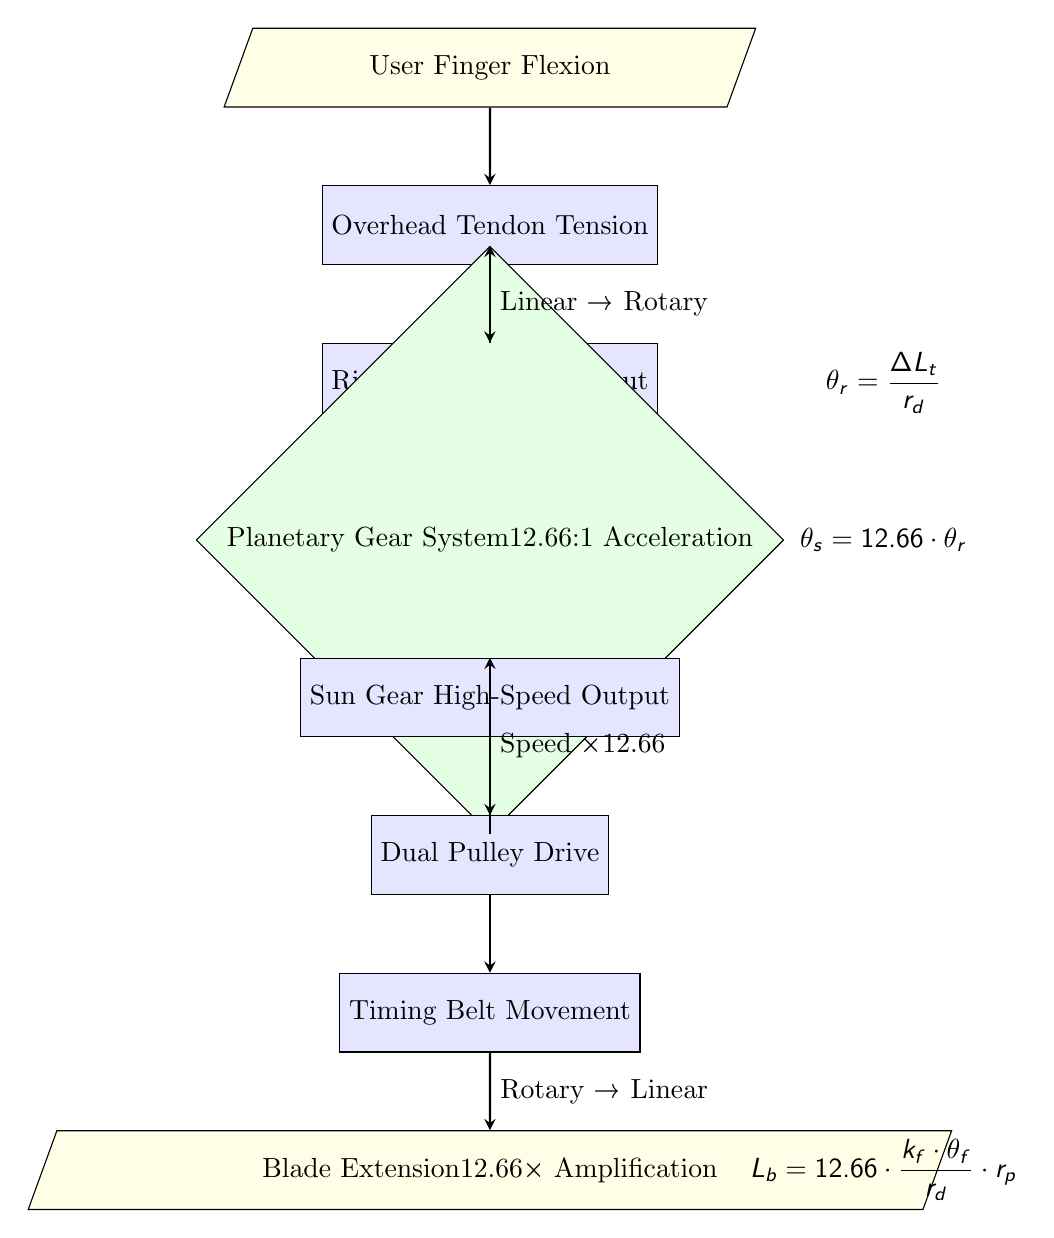
\begin{tikzpicture}[scale=0.8]
    % Define styles
    \tikzstyle{process} = [rectangle, minimum width=3cm, minimum height=1cm, text centered, draw=black, fill=blue!10]
    \tikzstyle{decision} = [diamond, minimum width=3cm, minimum height=1cm, text centered, draw=black, fill=green!10]
    \tikzstyle{io} = [trapezium, trapezium left angle=70, trapezium right angle=110, minimum width=3cm, minimum height=1cm, text centered, draw=black, fill=yellow!10]
    \tikzstyle{arrow} = [thick,->,>=stealth]
    
    % Nodes
    \node (start) [io] {User Finger Flexion};
    \node (tendon) [process, below of=start, yshift=-1cm] {Overhead Tendon Tension};
    \node (ring) [process, below of=tendon, yshift=-1cm] {Ring Gear Rotation Input};
    \node (planetary) [decision, below of=ring, yshift=-1cm] {Planetary Gear System\\12.66:1 Acceleration};
    \node (sun) [process, below of=planetary, yshift=-1cm] {Sun Gear High-Speed Output};
    \node (pulley) [process, below of=sun, yshift=-1cm] {Dual Pulley Drive};
    \node (belt) [process, below of=pulley, yshift=-1cm] {Timing Belt Movement};
    \node (blade) [io, below of=belt, yshift=-1cm] {Blade Extension\\12.66× Amplification};
    
    % Arrows
    \draw [arrow] (start) -- (tendon);
    \draw [arrow] (tendon) -- node[right] {Linear → Rotary} (ring);
    \draw [arrow] (ring) -- (planetary);
    \draw [arrow] (planetary) -- node[right] {Speed ×12.66} (sun);
    \draw [arrow] (sun) -- (pulley);
    \draw [arrow] (pulley) -- (belt);
    \draw [arrow] (belt) -- node[right] {Rotary → Linear} (blade);
    
    % Kinematic equations
    \node (eq1) [right of=ring, xshift=4cm] {$\theta_r = \dfrac{\Delta L_t}{r_d}$};
    \node (eq2) [right of=planetary, xshift=4cm] {$\theta_s = 12.66 \cdot \theta_r$};
    \node (eq3) [right of=blade, xshift=4cm] {$L_b = 12.66 \cdot \dfrac{k_f \cdot \theta_f}{r_d} \cdot r_p$};
\end{tikzpicture}

\subsubsection{Transmission Process Details}

\begin{enumerate}
    \item \textbf{Biomechanical Input (Finger Flexion)}: 
    \begin{itemize}
        \item Natural finger flexion creates geometric displacement
        \item Overhead tendon routing on finger dorsal side
        \item Tendon displacement: $\Delta L_t = k_f \cdot \theta_f$
    \end{itemize}
    
    \item \textbf{Tendon to Rotary Conversion}:
    \begin{itemize}
        \item Tendon wraps around drum connected to ring gear
        \item Linear displacement converted to rotational input
        \item Ring gear rotation: $\theta_r = \dfrac{\Delta L_t}{r_d}$
    \end{itemize}
    
    \item \textbf{Planetary Gear Acceleration}:
    \begin{itemize}
        \item Ring gear serves as input (unconventional configuration)
        \item Planet gears transfer motion to sun gear
        \item 12.66:1 acceleration ratio: $\theta_s = 12.66 \cdot \theta_r$
        \item Sun gear outputs high-speed, low-torque rotation
    \end{itemize}
    
    \item \textbf{Pulley and Belt Transmission}:
    \begin{itemize}
        \item Sun gear shaft drives dual synchronized pulleys
        \item Timing belts maintain parallel blade alignment
        \item Three blades mounted perpendicular between belts
    \end{itemize}
    
    \item \textbf{Final Blade Deployment}:
    \begin{itemize}
        \item Belt movement translates to linear blade extension
        \item Total amplification: 12.66× finger movement
        \item Final extension: $L_b = 12.66 \cdot \dfrac{k_f \cdot \theta_f}{r_d} \cdot r_p$
    \end{itemize}
\end{enumerate}

\subsubsection{Key Design Advantages}

\begin{itemize}
    \item \textbf{Amplification Efficiency}: 12.66× mechanical advantage enables significant blade extension from subtle finger movements
    \item \textbf{Compact Design}: Planetary gear system provides high ratio in minimal space
    \item \textbf{Intuitive Control}: Direct relationship between finger position and blade extension
    \item \textbf{Safety}: Acceleration mechanism requires minimal finger force, reducing user fatigue
\end{itemize}

\subsubsection{Kinematic Performance}

The complete transmission system achieves:
\begin{equation}
\text{Overall Ratio} = \underbrace{\frac{k_f}{r_d}}_{\text{Tendon}} \times \underbrace{12.66}_{\text{Planetary}} \times \underbrace{r_p}_{\text{Pulley}} = 12.66 \cdot \frac{k_f \cdot r_p}{r_d}
\end{equation}

Where small finger movements ($\theta_f$) result in proportionally larger blade extensions ($L_b$), making the system both responsive and precise for its intended applications.

This acceleration-based transmission represents an innovative approach to exoskeleton tool deployment, leveraging planetary gear mechanics to amplify natural human movements into effective tool operations.
\subsection{Fingers and Wrist Mechanisms}
\subsection{Wolf Claw Mechanism Comparison}
\subsubsection{Version 1: Planetary Gear}
\subsubsection{Version 2: Compound Gear Train}


\section{Mathematical Modelling and Analysis}
\subsection{Fingers and Wrist Modelling}
\subsection{Wolf Claw Mechanism \- Version 1: Planetary Gear}
\subsection{Wolf Claw Mechanism \- Version 2: Compound Gear Train}

\section{Conclusion and Future Work}

\pagebreak

\bibliographystyle{plain}
\bibliography{references}

\end{document}
